%%%%%%%%%%%%%%%%%%%%%%%%%%%%%%%%%%%%%%%%%
% The Legrand Orange Book
% LaTeX Template
% Version 2.1.1 (14/2/16)
%
% This template has been downloaded from:
% http://www.LaTeXTemplates.com
% https://pt.overleaf.com/latex/templates/the-legrand-orange-book-template-english/jtctyfmnpppc
%
% Original author:
% Mathias Legrand (legrand.mathias@gmail.com) with modifications by:
% Vel (vel@latextemplates.com)
%
%  License:
%  CC BY-NC-SA 3.0 (http://creativecommons.org/licenses/by-nc-sa/3.0/)
%
% Compiling this template:
% This template uses biber for its bibliography and makeindex for its index.
% When you first open the template, compile it from the command line with the 
% commands below to make sure your LaTeX distribution is configured correctly:
%
% 1) pdflatex main
% 2) makeindex main.idx -s StyleInd.ist
% 3) biber main
% 4) pdflatex main x 2
%
% After this, when you wish to update the bibliography/index use the appropriate
% command above and make sure to compile with pdflatex several times 
% afterwards to propagate your changes to the document.
%
% This template also uses a number of packages which may need to be
% updated to the newest versions for the template to compile. It is strongly
% recommended you update your LaTeX distribution if you have any
% compilation errors.
%
% Important note:
% Chapter heading images should have a 2:1 width:height ratio,
% e.g. 920px width and 460px height.
%
%%%%%%%%%%%%%%%%%%%%%%%%%%%%%%%%%%%%%%%%%

%----------------------------------------------------------------------------------------
%	 PACKAGES AND OTHER DOCUMENT CONFIGURATIONS
%----------------------------------------------------------------------------------------

\documentclass[11pt,fleqn]{book} % Default font size and left-justified equations

\usepackage{ccicons}

%----------------------------------------------------------------------------------------

%%%%%%%%%%%%%%%%%%%%%%%%%%%%%%%%%%%%%%%%%
% The Legrand Orange Book
% Structural Definitions File
% Version 2.0 (9/2/15)
%
% Original author:
% Mathias Legrand (legrand.mathias@gmail.com) with modifications by:
% Vel (vel@latextemplates.com)
% 
% This file has been downloaded from:
% http://www.LaTeXTemplates.com
%
%  License:
%  CC BY-NC-SA 3.0 (http://creativecommons.org/licenses/by-nc-sa/3.0/)
%
%%%%%%%%%%%%%%%%%%%%%%%%%%%%%%%%%%%%%%%%%

%----------------------------------------------------------------------------------------
% 	VARIOUS REQUIRED PACKAGES AND CONFIGURATIONS
%----------------------------------------------------------------------------------------

\usepackage[top=3cm,bottom=3cm,left=3cm,right=3cm,headsep=10pt,a4paper]{geometry} % Page margins

\usepackage{graphicx} % Required for including pictures
\graphicspath{{Pictures/}} % Specifies the directory where pictures are stored

\usepackage{lipsum} % Inserts dummy text

\usepackage{tikz} % Required for drawing custom shapes

\usepackage[brazil]{babel} % Brazilian Portuguese language/hyphenation

\usepackage{enumitem} % Customize lists
\setlist{nolistsep} % Reduce spacing between bullet points and numbered lists

\usepackage{booktabs} % Required for nicer horizontal rules in tables

\usepackage{xcolor} % Required for specifying colors by name
\definecolor{ocre}{RGB}{243,102,25} % Define the orange color used for highlighting throughout the book

%----------------------------------------------------------------------------------------
% 	FONTS
%----------------------------------------------------------------------------------------

\usepackage{avant} % Use the Avantgarde font for headings
%\usepackage{times} % Use the Times font for headings
\usepackage{mathptmx} % Use the Adobe Times Roman as the default text font together with math symbols from the Sym­bol, Chancery and Com­puter Modern fonts

\usepackage{microtype} % Slightly tweak font spacing for aesthetics
\usepackage[utf8]{inputenc} % Required for including letters with accents
\usepackage[T1]{fontenc} % Use 8-bit encoding that has 256 glyphs

%----------------------------------------------------------------------------------------
% 	BIBLIOGRAPHY AND INDEX
%----------------------------------------------------------------------------------------

\usepackage{csquotes}
\usepackage[style=abnt,citestyle=numeric,sorting=nyt,sortcites=true,autopunct=true,autolang=hyphen,hyperref=true,abbreviate=false,backref=true,backend=biber,defernumbers=true]{biblatex}
\addbibresource{bibliography.bib} % BibTeX bibliography file
\defbibheading{bibempty}{}

\usepackage{calc} % For simpler calculation - used for spacing the index letter headings correctly
\usepackage{makeidx} % Required to make an index
\makeindex % Tells LaTeX to create the files required for indexing

%----------------------------------------------------------------------------------------
% 	MAIN TABLE OF CONTENTS
%----------------------------------------------------------------------------------------

\usepackage{titletoc} % Required for manipulating the table of contents

\contentsmargin{0cm} % Removes the default margin

% Part text styling
\titlecontents{part}[0cm]
{\addvspace{20pt}\centering\large\bfseries}
{}
{}
{}

% Chapter text styling
\titlecontents{chapter}[1.25cm] % Indentation
{\addvspace{12pt}\large\sffamily\bfseries} % Spacing and font options for chapters
{\color{ocre!60}\contentslabel[\Large\thecontentslabel]{1.25cm}\color{ocre}} % Chapter number
{\color{ocre}}  
{\color{ocre!60}\normalsize\;\titlerule*[.5pc]{.}\;\thecontentspage} % Page number

% Section text styling
\titlecontents{section}[1.25cm] % Indentation
{\addvspace{3pt}\sffamily\bfseries} % Spacing and font options for sections
{\contentslabel[\thecontentslabel]{1.25cm}} % Section number
{}
{\hfill\color{black}\thecontentspage} % Page number
[]

% Subsection text styling
\titlecontents{subsection}[1.25cm] % Indentation
{\addvspace{1pt}\sffamily\small} % Spacing and font options for subsections
{\contentslabel[\thecontentslabel]{1.25cm}} % Subsection number
{}
{\ \titlerule*[.5pc]{.}\;\thecontentspage} % Page number
[]

% List of figures
\titlecontents{figure}[0em]
{\addvspace{-5pt}\sffamily}
{\thecontentslabel\hspace*{1em}}
{}
{\ \titlerule*[.5pc]{.}\;\thecontentspage}
[]

% List of tables
\titlecontents{table}[0em]
{\addvspace{-5pt}\sffamily}
{\thecontentslabel\hspace*{1em}}
{}
{\ \titlerule*[.5pc]{.}\;\thecontentspage}
[]

%----------------------------------------------------------------------------------------
% 	MINI TABLE OF CONTENTS IN PART HEADS
%----------------------------------------------------------------------------------------

% Chapter text styling
\titlecontents{lchapter}[0em] % Indenting
{\addvspace{15pt}\large\sffamily\bfseries} % Spacing and font options for chapters
{\color{ocre}\contentslabel[\Large\thecontentslabel]{1.25cm}\color{ocre}} % Chapter number
{}  
{\color{ocre}\normalsize\sffamily\bfseries\;\titlerule*[.5pc]{.}\;\thecontentspage} % Page number

% Section text styling
\titlecontents{lsection}[0em] % Indenting
{\sffamily\small} % Spacing and font options for sections
{\contentslabel[\thecontentslabel]{1.25cm}} % Section number
{}
{}

% Subsection text styling
\titlecontents{lsubsection}[.5em] % Indentation
{\normalfont\footnotesize\sffamily} % Font settings
{}
{}
{}

%----------------------------------------------------------------------------------------
% 	PAGE HEADERS
%----------------------------------------------------------------------------------------

\usepackage{fancyhdr} % Required for header and footer configuration

\pagestyle{fancy}
\renewcommand{\chaptermark}[1]{\markboth{\sffamily\normalsize\bfseries\chaptername\ \thechapter.\ #1}{}} % Chapter text font settings
\renewcommand{\sectionmark}[1]{\markright{\sffamily\normalsize\thesection\hspace{5pt}#1}{}} % Section text font settings
\fancyhf{} \fancyhead[LE,RO]{\sffamily\normalsize\thepage} % Font setting for the page number in the header
\fancyhead[LO]{\rightmark} % Print the nearest section name on the left side of odd pages
\fancyhead[RE]{\leftmark} % Print the current chapter name on the right side of even pages
\renewcommand{\headrulewidth}{0.5pt} % Width of the rule under the header
\addtolength{\headheight}{2.5pt} % Increase the spacing around the header slightly
\renewcommand{\footrulewidth}{0pt} % Removes the rule in the footer
\fancypagestyle{plain}{\fancyhead{}\renewcommand{\headrulewidth}{0pt}} % Style for when a plain pagestyle is specified

% Removes the header from odd empty pages at the end of chapters
\makeatletter
\renewcommand{\cleardoublepage}{
\clearpage\ifodd\c@page\else
\hbox{}
\vspace*{\fill}
\thispagestyle{empty}
\newpage
\fi}

%----------------------------------------------------------------------------------------
% 	THEOREM STYLES
%----------------------------------------------------------------------------------------

\usepackage{amsmath,amsfonts,amssymb,amsthm} % For math equations, theorems, symbols, etc

\newcommand{\intoo}[2]{\mathopen{]}#1\,;#2\mathclose{[}}
\newcommand{\ud}{\mathop{\mathrm{{}d}}\mathopen{}}
\newcommand{\intff}[2]{\mathopen{[}#1\,;#2\mathclose{]}}
\newtheorem{notation}{Notation}[chapter]

% Boxed/framed environments
\newtheoremstyle{ocrenumbox}% % Theorem style name
{0pt}% Space above
{0pt}% Space below
{\normalfont}% % Body font
{}% Indent amount
{\small\bf\sffamily\color{ocre}}% % Theorem head font
{\;}% Punctuation after theorem head
{0.25em}% Space after theorem head
{\small\sffamily\color{ocre}\thmname{#1}\nobreakspace\thmnumber{\@ifnotempty{#1}{}\@upn{#2}}% Theorem text (e.g. Theorem 2.1)
\thmnote{\nobreakspace\the\thm@notefont\sffamily\bfseries\color{black}---\nobreakspace#3.}} % Optional theorem note
\renewcommand{\qedsymbol}{$\blacksquare$}% Optional qed square

\newtheoremstyle{blacknumex}% Theorem style name
{5pt}% Space above
{5pt}% Space below
{\normalfont}% Body font
{} % Indent amount
{\small\bf\sffamily}% Theorem head font
{\;}% Punctuation after theorem head
{0.25em}% Space after theorem head
{\small\sffamily{\tiny\ensuremath{\blacksquare}}\nobreakspace\thmname{#1}\nobreakspace\thmnumber{\@ifnotempty{#1}{}\@upn{#2}}% Theorem text (e.g. Theorem 2.1)
\thmnote{\nobreakspace\the\thm@notefont\sffamily\bfseries---\nobreakspace#3.}}% Optional theorem note

\newtheoremstyle{blacknumbox} % Theorem style name
{0pt}% Space above
{0pt}% Space below
{\normalfont}% Body font
{}% Indent amount
{\small\bf\sffamily}% Theorem head font
{\;}% Punctuation after theorem head
{0.25em}% Space after theorem head
{\small\sffamily\thmname{#1}\nobreakspace\thmnumber{\@ifnotempty{#1}{}\@upn{#2}}% Theorem text (e.g. Theorem 2.1)
\thmnote{\nobreakspace\the\thm@notefont\sffamily\bfseries---\nobreakspace#3.}}% Optional theorem note

% Non-boxed/non-framed environments
\newtheoremstyle{ocrenum}% % Theorem style name
{5pt}% Space above
{5pt}% Space below
{\normalfont}% % Body font
{}% Indent amount
{\small\bf\sffamily\color{ocre}}% % Theorem head font
{\;}% Punctuation after theorem head
{0.25em}% Space after theorem head
{\small\sffamily\color{ocre}\thmname{#1}\nobreakspace\thmnumber{\@ifnotempty{#1}{}\@upn{#2}}% Theorem text (e.g. Theorem 2.1)
\thmnote{\nobreakspace\the\thm@notefont\sffamily\bfseries\color{black}---\nobreakspace#3.}} % Optional theorem note
\renewcommand{\qedsymbol}{$\blacksquare$}% Optional qed square
\makeatother

% Defines the theorem text style for each type of theorem to one of the three styles above
\newcounter{dummy} 
\numberwithin{dummy}{section}
\theoremstyle{ocrenumbox}
\newtheorem{theoremeT}[dummy]{Theorem}
\newtheorem{problem}{Problem}[chapter]
\newtheorem{exerciseT}{Exercise}[chapter]
\theoremstyle{blacknumex}
\newtheorem{exampleT}{Example}[chapter]
\theoremstyle{blacknumbox}
\newtheorem{vocabulary}{Vocabulary}[chapter]
\newtheorem{definitionT}{Definition}[section]
\newtheorem{corollaryT}[dummy]{Corollary}
\theoremstyle{ocrenum}
\newtheorem{proposition}[dummy]{Proposition}

%----------------------------------------------------------------------------------------
% 	DEFINITION OF COLORED BOXES
%----------------------------------------------------------------------------------------

\RequirePackage[framemethod=default]{mdframed} % Required for creating the theorem, definition, exercise and corollary boxes

% Theorem box
\newmdenv[skipabove=7pt,
skipbelow=7pt,
backgroundcolor=black!5,
linecolor=ocre,
innerleftmargin=5pt,
innerrightmargin=5pt,
innertopmargin=5pt,
leftmargin=0cm,
rightmargin=0cm,
innerbottommargin=5pt]{tBox}

% Exercise box	  
\newmdenv[skipabove=7pt,
skipbelow=7pt,
rightline=false,
leftline=true,
topline=false,
bottomline=false,
backgroundcolor=ocre!10,
linecolor=ocre,
innerleftmargin=5pt,
innerrightmargin=5pt,
innertopmargin=5pt,
innerbottommargin=5pt,
leftmargin=0cm,
rightmargin=0cm,
linewidth=4pt]{eBox}	

% Definition box
\newmdenv[skipabove=7pt,
skipbelow=7pt,
rightline=false,
leftline=true,
topline=false,
bottomline=false,
linecolor=ocre,
innerleftmargin=5pt,
innerrightmargin=5pt,
innertopmargin=0pt,
leftmargin=0cm,
rightmargin=0cm,
linewidth=4pt,
innerbottommargin=0pt]{dBox}	

% Corollary box
\newmdenv[skipabove=7pt,
skipbelow=7pt,
rightline=false,
leftline=true,
topline=false,
bottomline=false,
linecolor=gray,
backgroundcolor=black!5,
innerleftmargin=5pt,
innerrightmargin=5pt,
innertopmargin=5pt,
leftmargin=0cm,
rightmargin=0cm,
linewidth=4pt,
innerbottommargin=5pt]{cBox}

% Creates an environment for each type of theorem and assigns it a theorem text style from the "Theorem Styles" section above and a colored box from above
\newenvironment{theorem}{\begin{tBox}\begin{theoremeT}}{\end{theoremeT}\end{tBox}}
\newenvironment{exercise}{\begin{eBox}\begin{exerciseT}}{\hfill{\color{ocre}\tiny\ensuremath{\blacksquare}}\end{exerciseT}\end{eBox}}				  
\newenvironment{definition}{\begin{dBox}\begin{definitionT}}{\end{definitionT}\end{dBox}}	
\newenvironment{example}{\begin{exampleT}}{\hfill{\tiny\ensuremath{\blacksquare}}\end{exampleT}}		
\newenvironment{corollary}{\begin{cBox}\begin{corollaryT}}{\end{corollaryT}\end{cBox}}	

%----------------------------------------------------------------------------------------
% 	REMARK ENVIRONMENT
%----------------------------------------------------------------------------------------

\newenvironment{remark}{\par\vspace{10pt}\small % Vertical white space above the remark and smaller font size
\begin{list}{}{
\leftmargin=35pt % Indentation on the left
\rightmargin=25pt}\item\ignorespaces % Indentation on the right
\makebox[-2.5pt]{\begin{tikzpicture}[overlay]
\node[draw=ocre!60,line width=1pt,circle,fill=ocre!25,font=\sffamily\bfseries,inner sep=2pt,outer sep=0pt] at (-15pt,0pt){\textcolor{ocre}{R}};\end{tikzpicture}} % Orange R in a circle
\advance\baselineskip -1pt}{\end{list}\vskip5pt} % Tighter line spacing and white space after remark

%----------------------------------------------------------------------------------------
% 	SECTION NUMBERING IN THE MARGIN
%----------------------------------------------------------------------------------------

\makeatletter
\renewcommand{\@seccntformat}[1]{\llap{\textcolor{ocre}{\csname the#1\endcsname}\hspace{1em}}}                    
\renewcommand{\section}{\@startsection{section}{1}{\z@}
{-4ex \@plus -1ex \@minus -.4ex}
{1ex \@plus.2ex }
{\normalfont\large\sffamily\bfseries}}
\renewcommand{\subsection}{\@startsection {subsection}{2}{\z@}
{-3ex \@plus -0.1ex \@minus -.4ex}
{0.5ex \@plus.2ex }
{\normalfont\sffamily\bfseries}}
\renewcommand{\subsubsection}{\@startsection {subsubsection}{3}{\z@}
{-2ex \@plus -0.1ex \@minus -.2ex}
{.2ex \@plus.2ex }
{\normalfont\small\sffamily\bfseries}}                        
\renewcommand\paragraph{\@startsection{paragraph}{4}{\z@}
{-2ex \@plus-.2ex \@minus .2ex}
{.1ex}
{\normalfont\small\sffamily\bfseries}}

%----------------------------------------------------------------------------------------
% 	PART HEADINGS
%----------------------------------------------------------------------------------------

% numbered part in the table of contents
\newcommand{\@mypartnumtocformat}[2]{%
\setlength\fboxsep{0pt}%
\noindent\colorbox{ocre!20}{\strut\parbox[c][.7cm]{\ecart}{\color{ocre!70}\Large\sffamily\bfseries\centering#1}}\hskip\esp\colorbox{ocre!40}{\strut\parbox[c][.7cm]{\linewidth-\ecart-\esp}{\Large\sffamily\centering#2}}}%
%%%%%%%%%%%%%%%%%%%%%%%%%%%%%%%%%%
% unnumbered part in the table of contents
\newcommand{\@myparttocformat}[1]{%
\setlength\fboxsep{0pt}%
\noindent\colorbox{ocre!40}{\strut\parbox[c][.7cm]{\linewidth}{\Large\sffamily\centering#1}}}%
%%%%%%%%%%%%%%%%%%%%%%%%%%%%%%%%%%
\newlength\esp
\setlength\esp{4pt}
\newlength\ecart
\setlength\ecart{1.2cm-\esp}
\newcommand{\thepartimage}{}%
\newcommand{\partimage}[1]{\renewcommand{\thepartimage}{#1}}%
\def\@part[#1]#2{%
\ifnum \c@secnumdepth >-2\relax%
\refstepcounter{part}%
\addcontentsline{toc}{part}{\texorpdfstring{\protect\@mypartnumtocformat{\thepart}{#1}}{\partname~\thepart\ ---\ #1}}
\else%
\addcontentsline{toc}{part}{\texorpdfstring{\protect\@myparttocformat{#1}}{#1}}%
\fi%
\startcontents%
\markboth{}{}%
{\thispagestyle{empty}%
\begin{tikzpicture}[remember picture,overlay]%
\node at (current page.north west){\begin{tikzpicture}[remember picture,overlay]%	
\fill[ocre!20](0cm,0cm) rectangle (\paperwidth,-\paperheight);
\node[anchor=north] at (4cm,-3.25cm){\color{ocre!40}\fontsize{220}{100}\sffamily\bfseries\@Roman\c@part}; 
\node[anchor=south east] at (\paperwidth-1cm,-\paperheight+1cm){\parbox[t][][t]{8.5cm}{
\printcontents{l}{0}{\setcounter{tocdepth}{1}}%
}};
\node[anchor=north east] at (\paperwidth-1.5cm,-3.25cm){\parbox[t][][t]{15cm}{\strut\raggedleft\color{white}\fontsize{30}{30}\sffamily\bfseries#2}};
\end{tikzpicture}};
\end{tikzpicture}}%
\@endpart}
\def\@spart#1{%
\startcontents%
\phantomsection
{\thispagestyle{empty}%
\begin{tikzpicture}[remember picture,overlay]%
\node at (current page.north west){\begin{tikzpicture}[remember picture,overlay]%	
\fill[ocre!20](0cm,0cm) rectangle (\paperwidth,-\paperheight);
\node[anchor=north east] at (\paperwidth-1.5cm,-3.25cm){\parbox[t][][t]{15cm}{\strut\raggedleft\color{white}\fontsize{30}{30}\sffamily\bfseries#1}};
\end{tikzpicture}};
\end{tikzpicture}}
\addcontentsline{toc}{part}{\texorpdfstring{%
\setlength\fboxsep{0pt}%
\noindent\protect\colorbox{ocre!40}{\strut\protect\parbox[c][.7cm]{\linewidth}{\Large\sffamily\protect\centering #1\quad\mbox{}}}}{#1}}%
\@endpart}
\def\@endpart{\vfil\newpage
\if@twoside
\if@openright
\null
\thispagestyle{empty}%
\newpage
\fi
\fi
\if@tempswa
\twocolumn
\fi}

%----------------------------------------------------------------------------------------
% 	CHAPTER HEADINGS
%----------------------------------------------------------------------------------------

% A switch to conditionally include a picture, implemented by  Christian Hupfer
\newif\ifusechapterimage
\usechapterimagetrue
\newcommand{\thechapterimage}{}%
\newcommand{\chapterimage}[1]{\ifusechapterimage\renewcommand{\thechapterimage}{#1}\fi}%
\def\@makechapterhead#1{%
{\parindent \z@ \raggedright \normalfont
\ifnum \c@secnumdepth >\m@ne
\if@mainmatter
\begin{tikzpicture}[remember picture,overlay]
\node at (current page.north west)
{\begin{tikzpicture}[remember picture,overlay]
\node[anchor=north west,inner sep=0pt] at (0,0) {\ifusechapterimage\includegraphics[width=\paperwidth]{\thechapterimage}\fi};
\draw[anchor=west] (\Gm@lmargin,-9cm) node [line width=2pt,rounded corners=15pt,draw=ocre,fill=white,fill opacity=0.5,inner sep=15pt]{\strut\makebox[22cm]{}};
\draw[anchor=west] (\Gm@lmargin+.3cm,-9cm) node {\huge\sffamily\bfseries\color{black}\thechapter. #1\strut};
\end{tikzpicture}};
\end{tikzpicture}
\else
\begin{tikzpicture}[remember picture,overlay]
\node at (current page.north west)
{\begin{tikzpicture}[remember picture,overlay]
\node[anchor=north west,inner sep=0pt] at (0,0) {\ifusechapterimage\includegraphics[width=\paperwidth]{\thechapterimage}\fi};
\draw[anchor=west] (\Gm@lmargin,-9cm) node [line width=2pt,rounded corners=15pt,draw=ocre,fill=white,fill opacity=0.5,inner sep=15pt]{\strut\makebox[22cm]{}};
\draw[anchor=west] (\Gm@lmargin+.3cm,-9cm) node {\huge\sffamily\bfseries\color{black}#1\strut};
\end{tikzpicture}};
\end{tikzpicture}
\fi\fi\par\vspace*{270\p@}}}

%-------------------------------------------

\def\@makeschapterhead#1{%
\begin{tikzpicture}[remember picture,overlay]
\node at (current page.north west)
{\begin{tikzpicture}[remember picture,overlay]
\node[anchor=north west,inner sep=0pt] at (0,0) {\ifusechapterimage\includegraphics[width=\paperwidth]{\thechapterimage}\fi};
\draw[anchor=west] (\Gm@lmargin,-9cm) node [line width=2pt,rounded corners=15pt,draw=ocre,fill=white,fill opacity=0.5,inner sep=15pt]{\strut\makebox[22cm]{}};
\draw[anchor=west] (\Gm@lmargin+.3cm,-9cm) node {\huge\sffamily\bfseries\color{black}#1\strut};
\end{tikzpicture}};
\end{tikzpicture}
\par\vspace*{270\p@}}
\makeatother

%----------------------------------------------------------------------------------------
% 	HYPERLINKS IN THE DOCUMENTS
%----------------------------------------------------------------------------------------

\usepackage{hyperref}
\hypersetup{hidelinks,colorlinks=false,breaklinks=true,urlcolor= ocre,bookmarksopen=false,pdftitle={Title},pdfauthor={Author}}
\usepackage{bookmark}
\bookmarksetup{
open,
numbered,
addtohook={%
\ifnum\bookmarkget{level}=0 % chapter
\bookmarksetup{bold}%
\fi
\ifnum\bookmarkget{level}=-1 % part
\bookmarksetup{color=ocre,bold}%
\fi
}
}
 % Insert the commands.tex file which contains the majority of the structure behind the template

\begin{document}

%----------------------------------------------------------------------------------------
%	 TITLE PAGE
%----------------------------------------------------------------------------------------

\begingroup
\thispagestyle{empty}
\begin{tikzpicture}[remember picture,overlay]
\coordinate [below=12cm] (midpoint) at (current page.north);
\node at (current page.north west)
{\begin{tikzpicture}[remember picture,overlay]
\node[anchor=north west,inner sep=0pt] at (0,0) {\includegraphics[width=\paperwidth]{2016-10-21_mdc_partida_l11}}; % Background image
\draw[anchor=north] (midpoint) node [fill=black!90!white,fill opacity=0.6,text opacity=1,inner sep=1cm]{\Huge\centering\bfseries\sffamily\parbox[c][][t]{\paperwidth}{\centering \textcolor{white}{Querem privatizar a CPTM. E agora?} \\[15pt] % Book title
{\Large \textcolor{white}{Um arsenal para discussão de problemas e parcerias público-privadas}}\\[20pt] % Subtitle
{\huge \textcolor{white}{Coletivo Metropolitano de Mobilidade Urbana}}}}; % Author name
\end{tikzpicture}};
\end{tikzpicture}
\vfill
\endgroup

%----------------------------------------------------------------------------------------
%	 COPYRIGHT PAGE
%----------------------------------------------------------------------------------------

\newpage
~\vfill
\thispagestyle{empty}

\noindent Alguns direitos reservados ao Coletivo Metropolitano de Mobilidade Urbana, 2019 \\ % Informações de direitos

\noindent \textsc{Publicação independente}\\ % Publicador

\noindent \textsc{medium.com/@commu}\\ %  URL

\vspace{2cm}

\noindent {\Huge \ccbync} \\

\noindent Licenciado sob a \textbf{Licença Creative Commons Atribuição-NãoComercial 3.0-NãoAdaptada} (doravante denominada ``LICENÇA''), regida pelos termos: (i) atribuição: você deve dar o crédito apropriado, prover um link para a LICENÇA e indicar se mudanças foram feitas. Você deve fazê-lo em qualquer circunstância razoável, mas de nenhuma maneira que sugira que o licenciante apoia você ou o seu uso; (ii) veto à comercialização: você não pode usar o material para fins comerciais e; (iii) veto à restrição: você não pode aplicar termos jurídicos ou medidas de caráter tecnológico que restrinjam legalmente outros de fazerem algo que a LICENÇA permita. Material fornecido \textsc{``no estado'', sem qualquer garantia ou condições de qualquer tipo}, em quaisquer circunstâncias \\ % Informações de licensiamento

\vspace{0.5cm}

\noindent \textit{Primeira impressão. Março de 2019} % Impressão/data da edição

%----------------------------------------------------------------------------------------
% 	SUMÁRIO/CONTEÚDO
%----------------------------------------------------------------------------------------

%\usechapterimagefalse % If you don't want to include a chapter image, use this to toggle images off - it can be enabled later with \usechapterimagetrue

\chapterimage{2012-12-21_vol_passarela_l9} % Table of contents heading image

\pagestyle{empty} % No headers

\tableofcontents % Print the table of contents itself

\cleardoublepage % Forces the first chapter to start on an odd page so it's on the right

\pagestyle{fancy} % Print headers again


%----------------------------------------------------------------------------------------
% 	PREFÁCIO
%----------------------------------------------------------------------------------------

\chapterimage{2016-04-13_bru_embarque_l8} % Imagem do cabeçalho do capítulo
\chapter*{Apresentação}\index{Apresentação}

\section*{Prefácio}

\lipsum[1-2]

\section*{Convenções}

Para facilitar a compreensão, algumas convenções são adotadas ao longo do livro:

\begin{info}
	Utilizado para fornecimento de informações adicionais, como dados de autorais.
\end{info}

\begin{obs}
	Observação: utilizado para salientar detalhes observados de forma particular pelo autor.
\end{obs}

%----------------------------------------------------------------------------------------
% 	PARTE 1
%----------------------------------------------------------------------------------------

\part{Contextualização}\index{Contextualização}

\chapterimage{2018-06-20_fmo_9500_l7} % Imagem do cabeçalho do capítulo
\chapter{A estatal}

\section{Surgimento da CPTM}

\lipsum[3-4]

\section{Evolução da demanda de passageiros}

\lipsum[3-4]

\section{Parceiras público-privadas em andamento}

\lipsum[3-4]

\section{Parceiras público-privadas fracassadas}

\lipsum[3-4]

\chapterimage{2019-02-09_est_passarela_l11} % Imagem do cabeçalho do capítulo
\chapter{O território atendido}

\section{Os municípios}

\lipsum[3-4]

\section{Potencialidades}

\lipsum[3-4]

\section{Eixos de desenvolvimento}

\lipsum[3-4]

\section{Habitação social em complexos de habitação intensiva}

\lipsum[3-4]

%----------------------------------------------------------------------------------------
% 	PARTE 2
%----------------------------------------------------------------------------------------

\part{Análise}

\chapterimage{2019-02-09_ego_sinal68} % Imagem do cabeçalho do capítulo
\chapter{Apropriando-se da infraestrutura}

\section{Estação Luz}

Imponente por fora, a estação vive hoje cenas de saturação, que muitas vezes levam a comportamentos no mínimo duvidosos (para não dizer arriscados) nos horários de pico. A estrutura, de arquitetura inglesa, revela uma rotina apressada, que por vezes sobrepõe-se a razão. A Estação da Luz merece viver melhores dias e, com ela, todos os passageiros e passageiras.

\subsection{Projeto Integração Centro}

Oficialmente, a CPTM informa como data de inauguração a data de 30/11/2004, a informação está contida na área de linhas do site\footnote{\url{https://www.cptm.sp.gov.br/sua-viagem/Pages/Linhas.aspx}}. O ano de 2004 está relacionado com o fracassado Projeto Integração Centro, uma tentativa de conexão entre as seis linhas da CPTM e o eixo central (Brás-Luz-Barra Funda), que na altura acabou subestimando a demanda dos subúrbios e o próprio papel do sistema de trilhos, que passava a ganhar contornos de malha integrada, algo que até então ainda não era tão enfatizado.

\begin{figure}[htb]
	\centering
	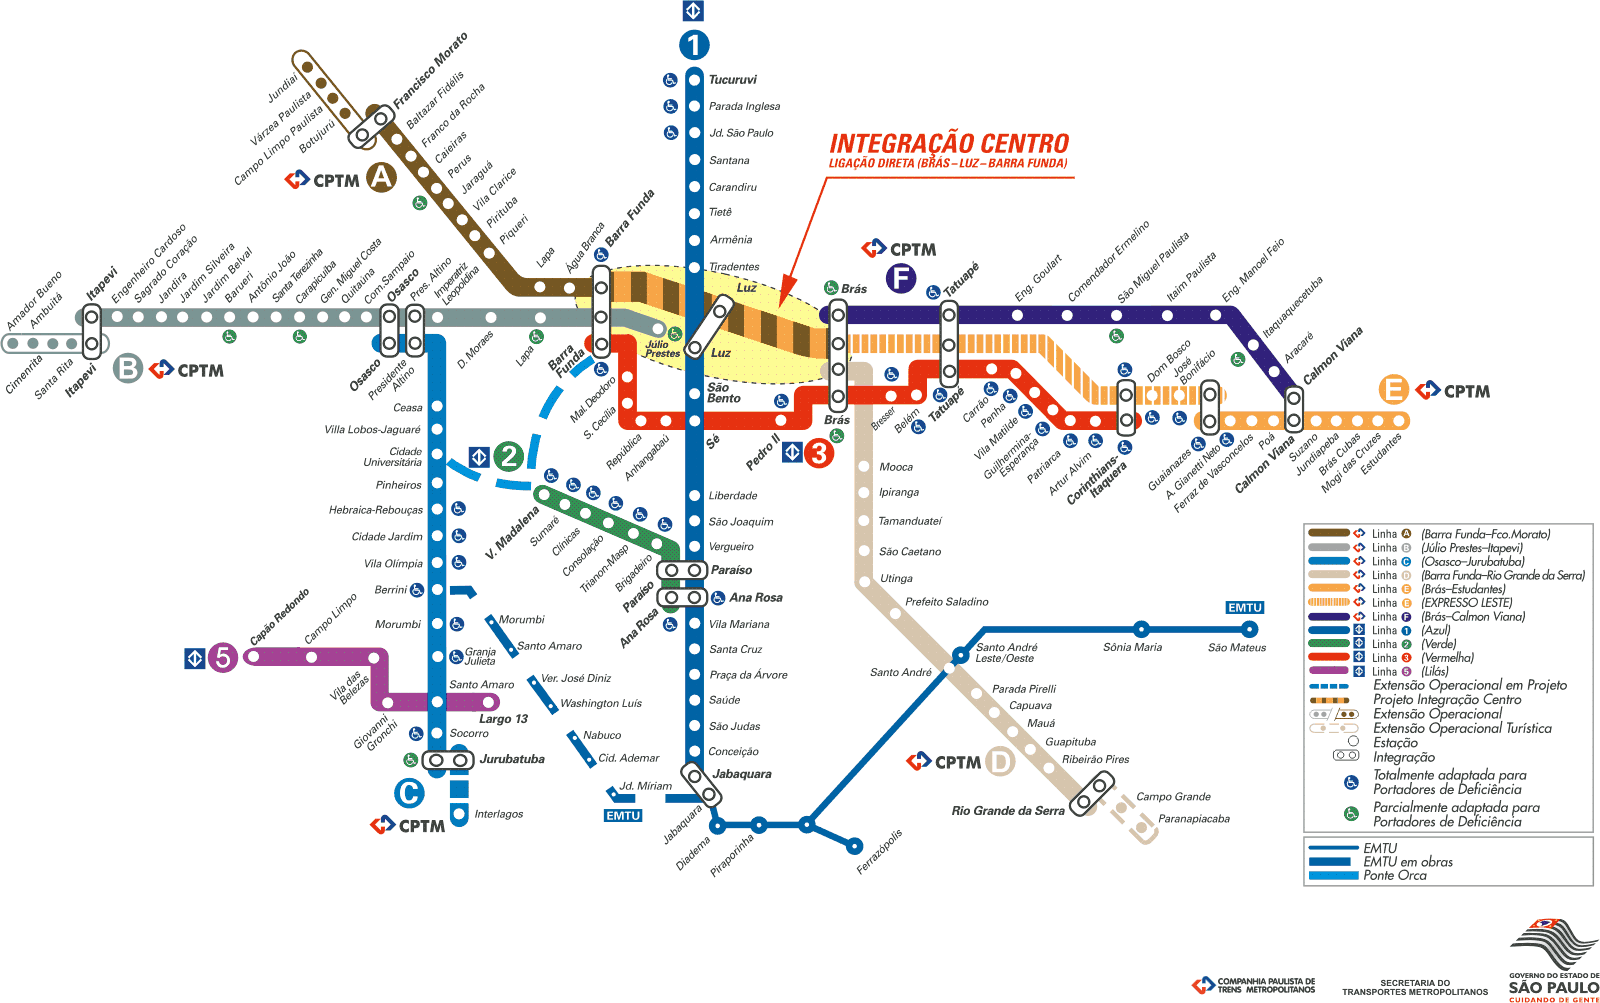
\includegraphics[width=\linewidth]{diagrama_integracao_centro}
	\caption[Mapa do Integração Centro]{Antigo mapa do transporte metropolitano, com o Integração Centro em destaque}
	\label{fig:diag_ic}
\end{figure}

Pagamos o preço pelas limitações oriundas do Integração Centro até os dias atuais. Corredores e acessos foram dimensionados para um universo em que o intervalo era de 10 minutos e a demanda das linhas da CPTM não chegava nem perto dos cerca de 3 milhões atuais. Projetos ruins no passado significam sofrimento por até uma década ou mais.

Mesmo com as limitações, é preciso mencionar que o projeto foi o responsável pelo corredor de integração entre a CPTM e o Metrô, indispensável nos dias atuais. Na época a estação também foi reformada e ao passar a contar com acessos subterrâneos, teve a plataforma central remodelada e ganhou novos sanitários.

\subsection{Transformações recentes}

Nos últimos 15 anos, a estação sofreu mudanças quanto às linhas disponíveis para embarque a partir dela. Abaixo podemos conferir quais linhas operam atualmente.

%TODO inserir tabela

Com a chegada da Linha 4-Amarela, o corredor de integração foi modificado, passando a contar com um novo acesso na lateral. Uma espécie de “desvio” foi feito na tentativa de organizar o fluxo nos horários de pico e a impressão de “puxadão” é inevitável. A integração, já saturada, ganhou ares de improviso.

Outro aspecto notável é que depois da chegada da Linha 4, a Linha 10 foi retirada da estação, passando a fazer terminal na Estação Brás. A operação das linhas 7 e 10 sempre foi ruim e, na verdade, a gare histórica de 1901 não foi pensada como terminal.

Simplesmente faltava uma plataforma adicional para viabilizar a operação que a CPTM tentava fazer. Como a operação era feita numa única plataforma para as linhas 7 e 10, chegou-se ao limite de maneira relativamente rápida e os seguintes fatores inviabilizadores surgiram:

\begin{itemize}
	\item Demanda crescente nas linhas da CPTM;
	\item Dificuldade de esvaziamento da plataforma central;
	\item Redução de intervalos nas linhas da CPTM;
	\item Chegada da Linha 4.
\end{itemize}

A CPTM decidiu, mesmo após realização de obras na via permanente, manter a Linha 10 no Brás. A decisão revoltou alguns passageiros e contrariou o informativo impresso que chegou a ser distribuído na época, como podemos ver na \autoref{fig:l10_luz}.

\begin{figure}[htb]
	\centering
	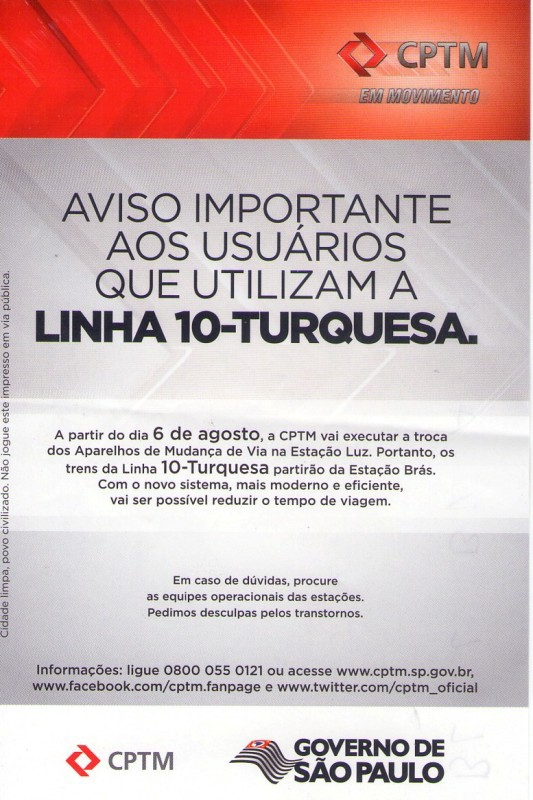
\includegraphics[width=\linewidth]{informativo_l10_luz}
	\caption[Informativo agosto/2011]{Informativo distribuído em agosto de 2011}
	\label{fig:l10_luz}
\end{figure}

Se observarmos os dados de demanda atuais fornecidos pela CPTM, temos o seguinte quadro, no qual a Linha 10 é a de menor demanda em média por dia útil.

%TODO inserir gráfico atualizado

\subsection{Projetos e mais projetos}

A mudança realizada na Linha 10, a despeito das obras e das promessas feitas aos usuários, parece ter sido uma decisão fruto da incapacidade de elaborar e cumprir bons planos, olhando para o caráter estruturante da malha. Verdade seja dita: a CPTM tem alguns projetos para o futuro, mas patina para tirá-los do papel. Vejamos\dots

\begin{itemize}
	\item Expandir a Linha 11 até a Estação Palmeiras-Barra Funda;
	\item Criar uma Linha 10 expressa (Expresso ABC), com terminal na Estação Palmeiras-Barra Funda;
	\item Construir uma nova estação de integração na região central (atualmente chamada de Bom Retiro, no local em que está a Favela do Moinho);
	\item Desativar a Estação Júlio Prestes (polêmico, ora dizem que irão desativar, ora voltam atrás).
\end{itemize}

%TODO foto do saguão da Luz

Para a expansão da Linha 11, obras foram realizadas entre as estações Luz e Palmeiras-Barra Funda, além disso, foram adquiridos 9 novos trens, cuja série atribuída é 9000 e cujo último trem (que na realidade foi o primeiro da série, o mais problemático) foi entregue recentemente pelo governador Geraldo Alckmin\footnote{\url{http://cptm.sp.gov.br/webnoticias/one_news.asp?IDNews=10148}}.

Sobre a futura Estação Bom Retiro, esta parece ser uma espécie de paliativo, fortalecido pelo fracasso da operação Nova Luz da gestão Kassab (prefeitura da capital). Previa-se para a região uma estação denominada Nova Luz, com plataformas subterrâneas, que não só serviria para desafogar a gare centenária, como também estaria ligada a um projeto ambicioso, visando tornar subterrâneos os trilhos da CPTM entre as regiões do Brás e da Lapa, eliminando gargalos históricos e estimulando uma ocupação melhor de áreas hoje ocupadas por galpões subutilizados.

Já com relação à Estação Júlio Prestes, em 07/02/2012 o jornal Estadão publicava matéria intitulada ``Superlotada, Estação Luz vai ter nova passarela e mais saídas de passageiros'' \footnote{\url{http://sao-paulo.estadao.com.br/noticias/geral,superlotada-estacao-luz-vai-ter-nova-passarela-e-mais-saidas-de-passageiros,832739}}, nela a intenção de integração outrora mencionada é revelada no último parágrafo:

\begin{citacao}
	A terceira mudança (tida como mais “embrionária” pelo governo do Estado) será a construção de um túnel entre as Estações Luz e Júlio Prestes. As paradas estão a cerca de 400 metros uma da outra, mas não têm conexão. A ideia é fazer uma passagem com esteiras rolantes, que poderiam ser usadas especialmente por pessoas que queiram ir à Sala São Paulo (na Júlio Prestes) e ao Museu da Língua Portuguesa (na Luz).
\end{citacao}

Como falamos no início, a Estação Luz sofreu diversas mudanças, mas infelizmente a vizinha Júlio Prestes não teve a mesma sorte e uma grande oportunidade foi desperdiçada, uma vez que não só a Estação Júlio Prestes continuou sem grandes modificações (até as placas internas são as mesmas da época da Fepasa), como também está isolada do restante do sistema de trilhos, uma vez que apenas a Linha 8-Diamante (Júlio Prestes-Itapevi-Amador Bueno) dá acesso à estação. Mais de 10 anos após o Projeto Integração Centro, ainda não há qualquer definição, a empresa parece ter engavetado de forma mesquinha e egoísta o projeto de enterramento dos trilhos, ao passo que também demonstra indecisão: não sabe se investe ou não na Estação Júlio Prestes, uma vez que no contexto de uma nova gare para a Estação Luz, a antiga estação da Sorocabana seria transformada em um centro de convenções.

\begin{figure}[htb]
	\centering
	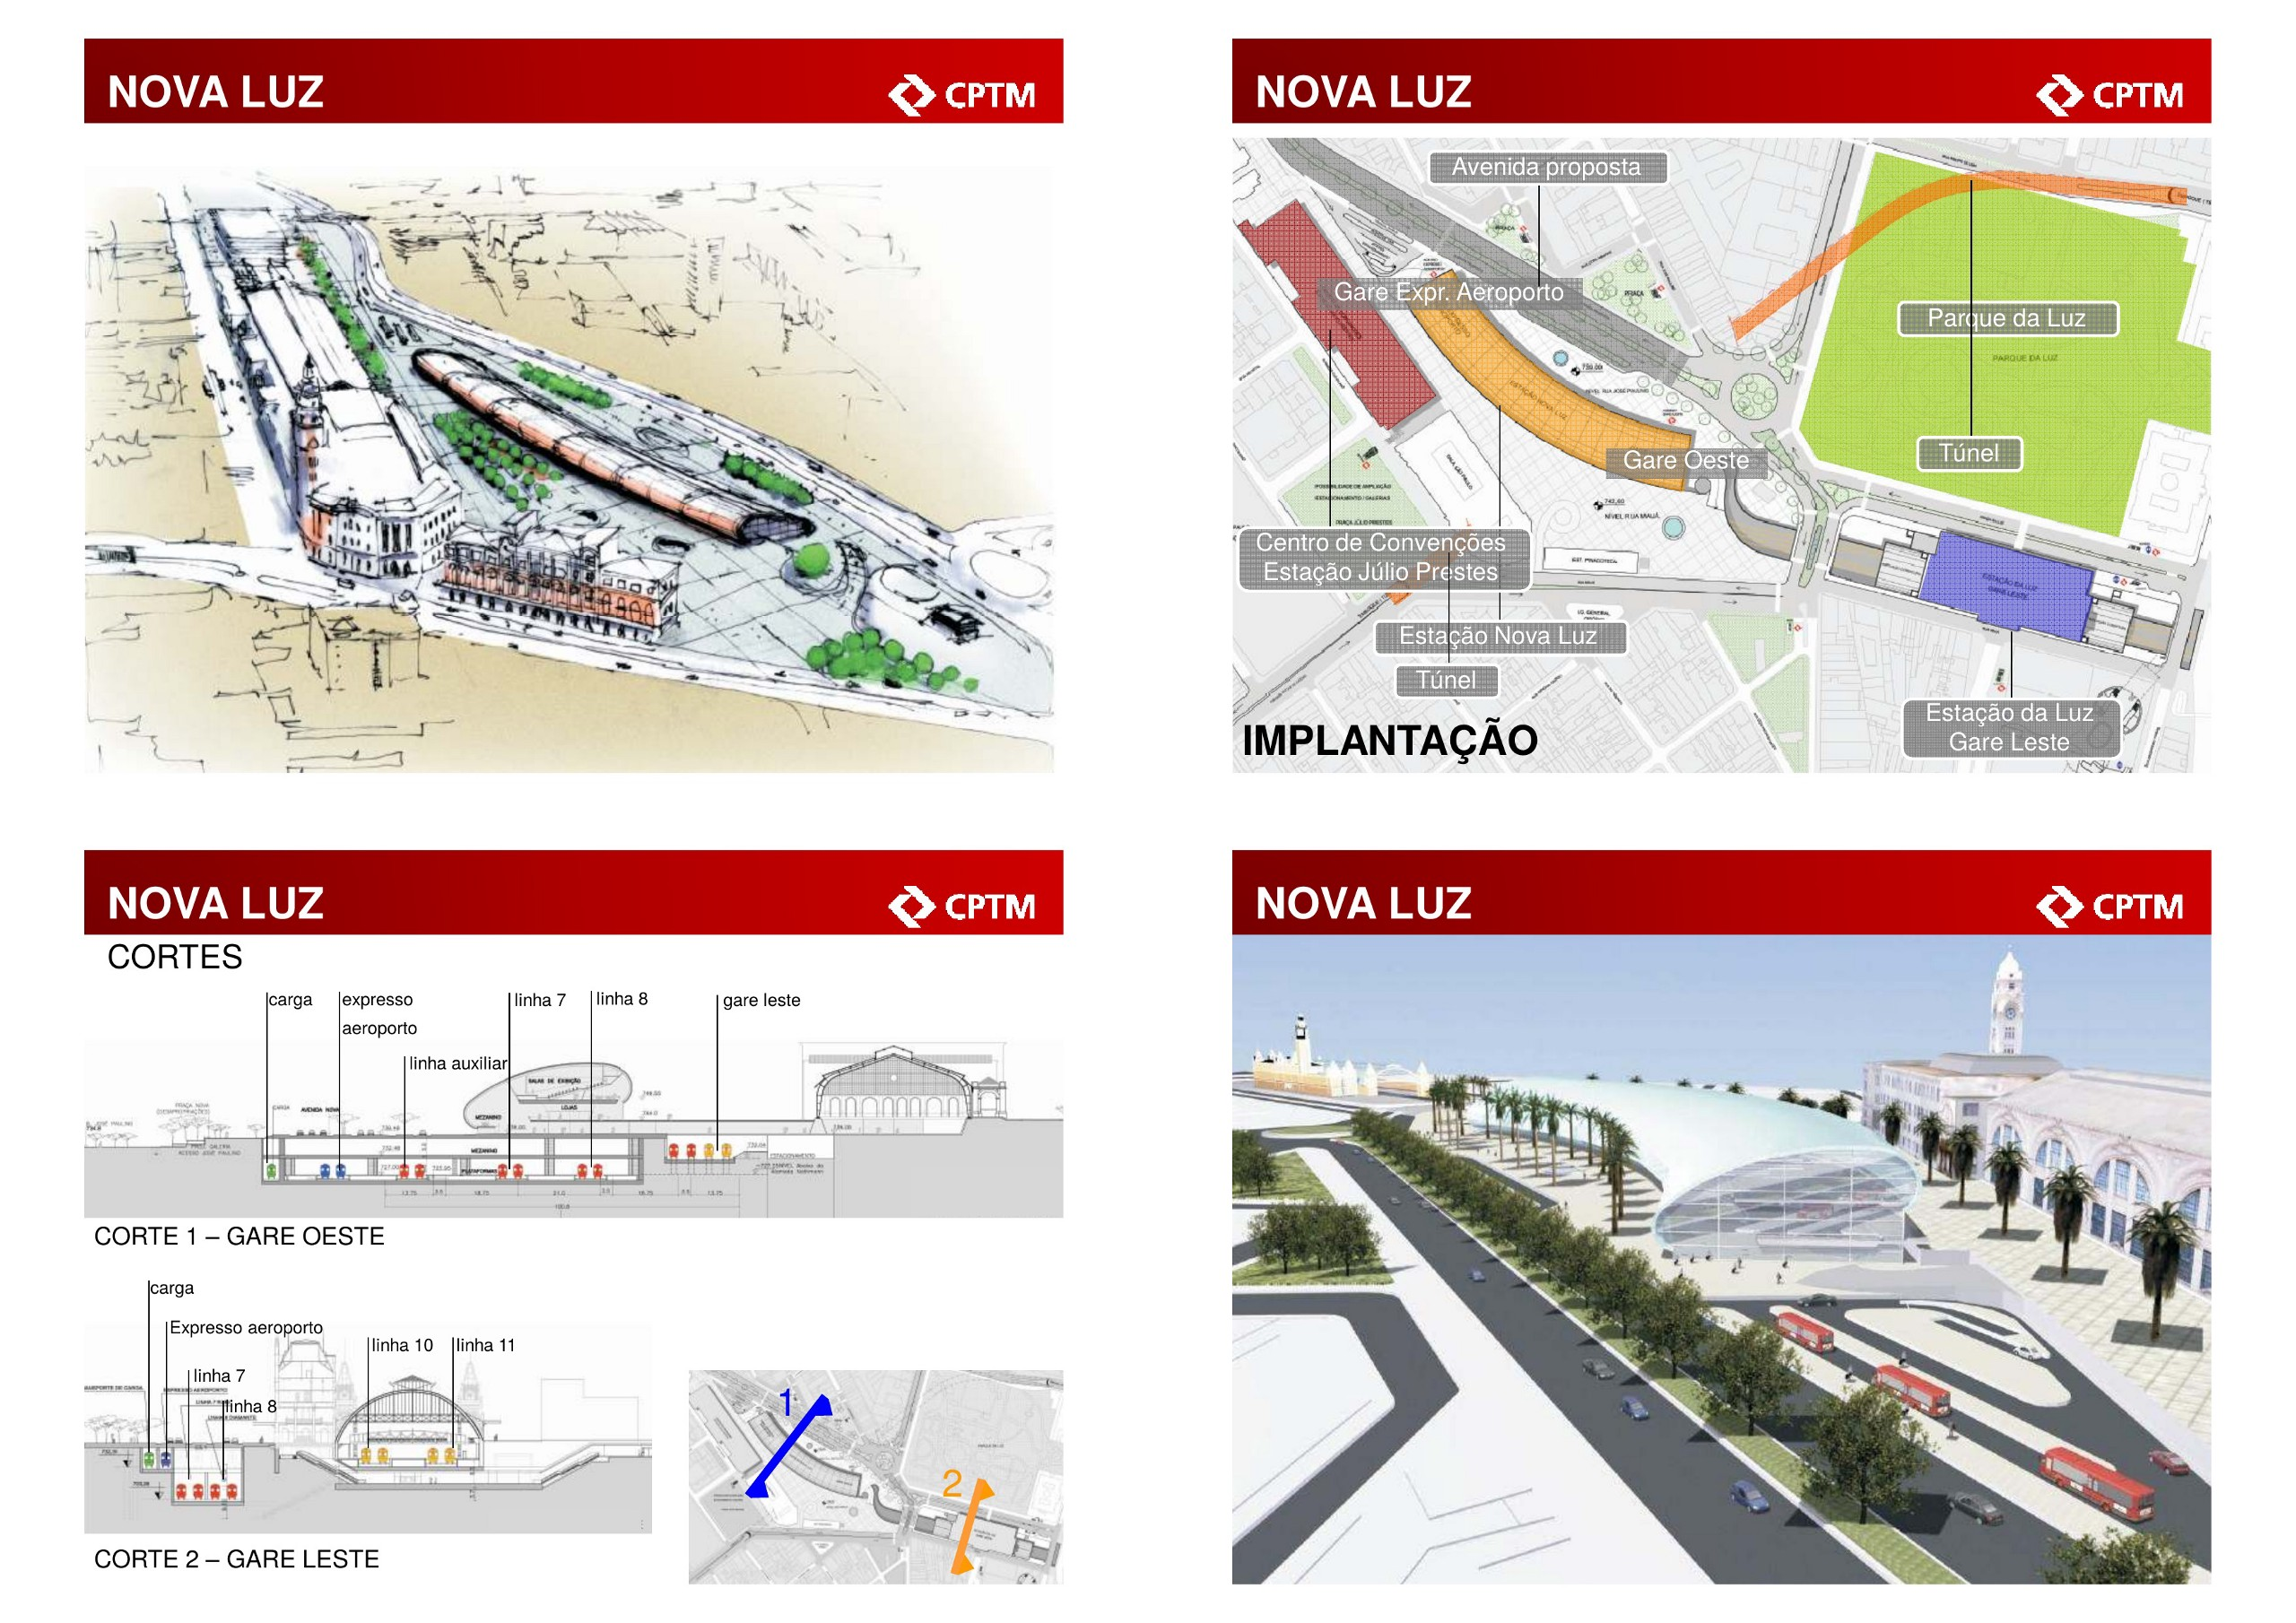
\includegraphics[width=\linewidth]{slides_nova_luz}
	\caption[Nova Luz conforme slides da CPTM para a AEAMESP]{Slides 112, 114, 116 e 116 de uma apresentação da CPTM realizada na AEAMESP\footnote{\url{http://web.archive.org/web/20101227091520/http://biblioteca.aeamesp.org.br/smns/16smtf100914pl102.pdf}}. Aqui podemos ter uma ideia de como seria a Nova Luz (Gare Oeste da Estação Luz)}
	\label{fig:slides_nova_luz}
\end{figure}

Pouco transparente, a CPTM não precisa datas para seus projetos, não publica cronogramas e não conduz pesquisas com usuários, também parece avessa à participação popular.

Comentamos sobre o projeto de enterramento dos trilhos feito pela Fupam em outro texto. Vale a pena conferir o vídeo do projeto, que permite ter uma visão rápida sobre a proposta:

%TODO ver o que fazer com o texto sobre os 130 km dentro da capital

\subsubsection{O pico}

O horário de pico na Estação Luz é ruim, ele se estende por horas, sendo possível evidenciar desconforto mesmo por volta das 19h. É possível afirmar que o pico já está consolidado por volta das 17h.

Podemos resumir os problemas da estação como sendo:

\begin{itemize}
	\item Embarque perigoso, uma vez que as plataformas laterais têm dimensão problemática, limitando a instalação de organizadores de fluxo. Uma situação ideal poderia implicar na instalação de portas de plataforma;
	\item Escadas insuficientes na plataforma central, tornando o desembarque no pico da manhã arriscado, uma vez que a plataforma não esvazia devido ao baixo intervalo praticado hoje (na Linha 11, beira os 4 minutos em média). Usuários não respeitam a faixa amarela e se arriscam a medida que os trens deixam a plataforma;
	\item Corredor de integração com dimensões reduzidas e com organização deficiente na chegada ao saguão da CPTM, com conflitos entre quem se dirige ao Metrô no contra-fluxo
	\item Nos picos a transferência entre as linhas 7-Rubi e 11-Coral pode ser desafiadora, uma vez que a maioria se dirige às linhas do Metrô;
	\item Buscando otimizar o fluxo do corredor de integração a CPTM fechou todas as lojas existentes, mas não liberou o espaço, reforçando o fracasso do projeto original
	\item O balcão de informações fica numa área ruim, muito próximo do acesso ao corredor de integração;
	\item A área livre da estação funciona como ponto de prostituição e a CPTM demonstra conivência, uma vez que não coíbe a prática mesmo em plena luz do dia.
\end{itemize}

No horário de pico filas se formam nas escadas de acesso às plataformas, principalmente na Linha 11. Como explicado, a plataforma tem dimensões limitadas os acessos a ela foram concebidos num cenário de demanda muito diferente do atual. Mesmo com o desligamento das escadas o acúmulo é inevitável.

É evidente que a CPTM não sabe mais o que fazer. Se ela tentar limitar o fluxo no corredor, ponto crítico, superlota a Estação Luz da Linha 1-Azul do Metrô. É crucial que a empresa pense numa gare adicional ou pelo menos um novo projeto integrador, contemplando a Estação Júlio Prestes. É o preço dos equívocos feitos anteriormente, que só aumenta com a manutenção do cenário.

\subsubsection{Conclusão}

A Estação Luz da CPTM é belíssima, um marco no Centro de São Paulo, que impressiona não só pela beleza de sua arquitetura centenária, mas também pela versatilidade proporcionada pelas conexões ali existentes. O problema é que o projeto que levou à sua restauração e modernização foi feito de maneira tacanha.

O plano diretor de inserção urbana da rede da CPTM, feito pela Fupam, bem como o projeto de enterramento, aparentemente foram demonstrações de que a estatal estava entrando nos trilhos, até que algo aconteceu e ela descarrilou. Kassab enfrentou dificuldades com o Nova Luz (nada surpreendentes pela forma como conduziu o processo), mas as dificuldades com o Nova Luz não poderiam, devido à questão dos CEPACs (certificados de potencial adicional de construção, que permitiram ao município angariar fundos para colocar no projeto de enterramento), motivar o engavetamento da parte que cabia à CPTM. É utópico, na conjuntura atual, esperar que a capital custeie fortemente o enterramento de uma infraestrutura que não pertence a ela, principalmente quando houve, para variar, passividade do Governo do Estado, que esperou cerca de 10 anos para pensar em algo, se mostrando incapaz de levar a empreitada adiante.

A superlotação e os gargalos na Estação da Luz \textemdash e também no eixo Brás-Lapa \textemdash só têm se agravado com a postura do governo estadual e da Secretaria dos Transportes Metropolitanos.

\begin{info}
	\textbf{Autor}: Caio César Carvalho Ortega \\
	\textbf{Originalmente publicado em:} 01/03/2015 \\
	\textbf{Endereço do original:} \url{https://medium.com/trens-metropolitanos/mar%C3%A7o-e-a-esta%C3%A7%C3%A3o-luz-m%C3%AAs-de-um-anivers%C3%A1rio-ingl%C3%B3rio-1f23e0adc672}
\end{info}

\section{Algum outro tema}

\begin{obs}
	Teste
\end{obs}

%----------------------------------------------------------------------------------------
% 	BIBLIOGRAFIA
%----------------------------------------------------------------------------------------

\chapterimage{2019-02-09_tat_plataforma_l12} % Imagem do cabeçalho do capítulo
\chapter*{Bibliografia}
\addcontentsline{toc}{chapter}{\textcolor{red}{Bibliografia}}
\section*{Livros}
\addcontentsline{toc}{section}{Livros}
\printbibliography[heading=bibempty,type=book]
\section*{Artigos}
\addcontentsline{toc}{section}{Artigos}
\printbibliography[heading=bibempty,type=article]

%----------------------------------------------------------------------------------------
% 	ÍNDICE
%----------------------------------------------------------------------------------------

\cleardoublepage
\phantomsection
\setlength{\columnsep}{0.75cm}
\chapterimage{2018-04-06_psa_arte_l10} % Imagem do cabeçalho do capítulo
\addcontentsline{toc}{chapter}{\textcolor{red}{Index}}
\printindex

%----------------------------------------------------------------------------------------

\end{document}
